%& --translate-file=utf8
\documentclass[a4paper,12pt]{article}
\usepackage[T1]{fontenc}
\usepackage[utf8]{inputenc}
\usepackage{graphicx}
\usepackage{hyperref}

\begin{document}

\title{Raport (I wersja) - Grammatical Facial Expression}
\author{Marek Parr, Michał Mitros}
\date{10.01.2020}
\maketitle

\newpage
Link do projekt na github.com:\\
\href{https://github.com/MichalMitros/GrammaticalFacialExpression}{https://github.com/MichalMitros/GrammaticalFacialExpression}
\section{Cel badania}
\hspace{1cm}Celem badania jest wyznaczenie modelu klasyfikatora zdolnego do odróżniania gestów na twarzy człowieka na podstawie zapisów z kamer \textsl{Microsoft Kinect} (kamer z sensorami głębi umożliwiających wyznaczenie trójwymiarowej mapy twarzy). Model powinien powstać w wyniku uczenia na podstawie dostarczonego zbioru danych \textsl{Grammatical Facial Expression}.

\section{Opis zbioru danych}
\hspace{1cm}Zbiór danych ma postać 18 par plików. Dane zostały stworzone w oparciu o nagrania dwóch osób wykonujących 9 gestów. Pierwszy plik danej pary zawiera w każdym wierszu czas zapisu (\textsl{timestamp}) oraz współrzędne (x, y, z) ponad 100 punktów na twarzy (oczy, nos, lewa brew, kontur twarzy, ...). W jednym pliku wiersze pochodzą z ok. 5 minut nagrania. Drugi plik pary zawiera etykiety wyznaczone ręcznie przez specjalistów (0 przy braku gestu, 1 podczas wykonywania gestu) w wierszach odpowiadających odpowiednim pozycjom w pierwszym pliku.\newline
Współrzędne X i Y mierzone są w pikselach i odpowiadają pikselowi na nagraniu. Współrzędna Z mierzona jest jako odległość danego punktu od sensora (w milimetrach).\newline

\hspace{1cm}Razem we wszystkich plikach jest 27936 rekordów, wśród których jest 9877 rekordów z jednoznacznie oznaczonym gestem. Pozostałe rekordy interpretować można jako "niewykonywanie jednego z gestów", ale nie wiadomo, czy są one "brakiem gestu", który można klasyfikować jako oddzielną klasę, czy być może niektóre z nich powinny być zaklasyfikowane jako jeden z gestów, inny, niż ten, którego dotyczył plik źródłowy rekordu. Żadna z klas znacząco nie przeważa, ani nie przegrywa pod względem liczności, rozkład atrybutów decyzyjnych nie wymusza uwzględniania mniej licznych klas.

\begin{center}
	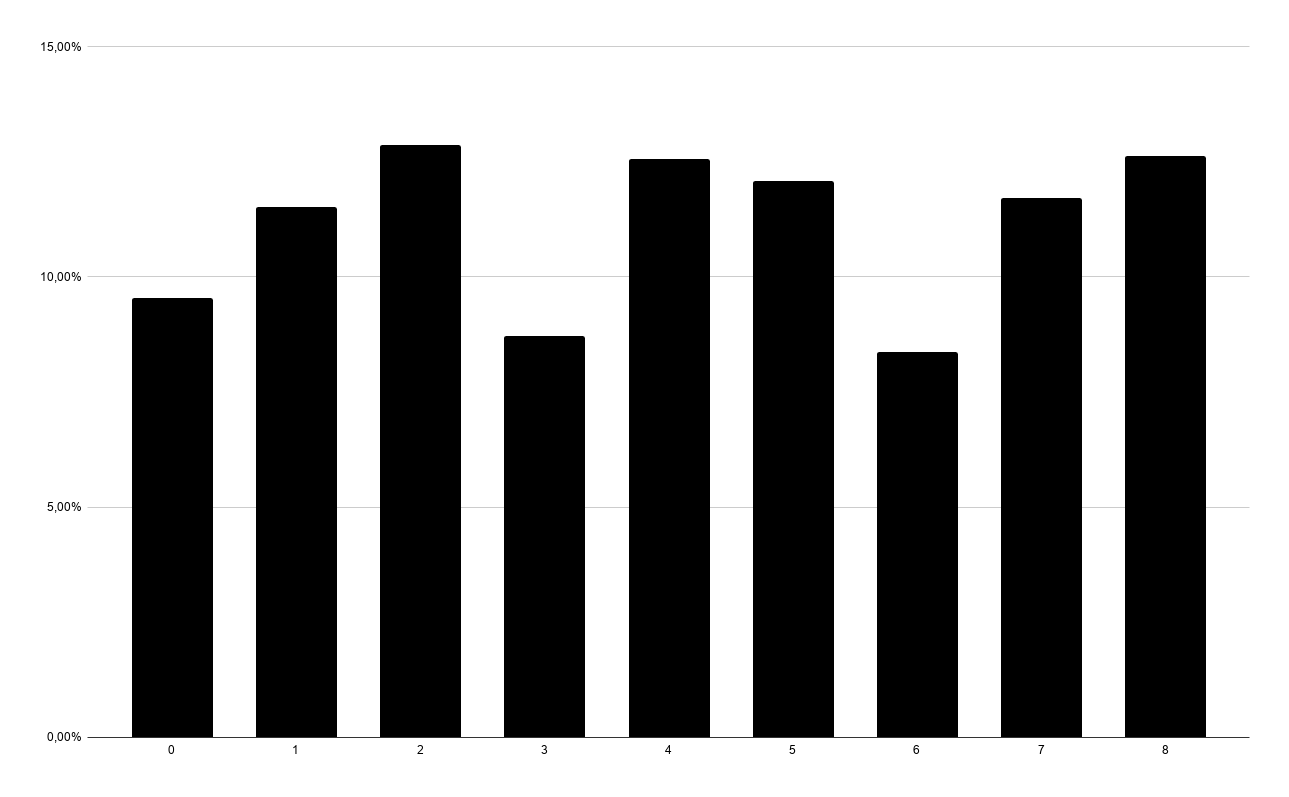
\includegraphics[scale=0.25]{rozklad.png}
	\\\small Rozkład klas decyzyjnych
	\\(0-8) - indeksy poszczególnych gestów
\end{center}

\section{Metodologia}
\hspace{1cm}Problem klasyfikacji rozwiązany będzie za pomocą sieci neuronowej. Sieć ma docelowo posiadać dwie warstwy ukryte, ale początkowo klasyfikator zostanie przetestowany z jedną warstwą ukrytą. Całość napisana zostanie w języku Python 3, a do utworzenia sieci posłuży biblioteka \textsl{numpy} dostarczająca potrzebne operacje na macierzach. Globalną funkcją aktywacji w sieci będzie sigmoid. Każdy neuron wejściowy będzie odpowiadał jednej współrzędnej składowej rekordu. Oznacza to, że sieć będzie miała ok. 300 neuronów wejściowych. Neuronów wyjściowych początkowo będzie 9 - każdy będzie interpretowany jako pojedyncza klasa. Ilość neuronów w warstwach ukrytych (obecnie jednej warstwie ukrytej) oraz wartość współczynnika uczenia (\textsl{learning rate}) będą dobrane metodą eksperymentów.

\section{Wstępne przetwarzanie danych}
\hspace{1cm}Pierwszym etapem będzie przygotowanie danych. Według źródła, z którego pochodzi zbiór, wśród atrybutów nie ma brakujących wartości, dlatego nie trzeba rozważać przypadku pustych kolumn. Pierwszym etapem preprocessingu jest konsolidacja plików z danymi, w wyniku której wszystkie rekordy znajdą się w jednym pliku. Z danych usunięta zostanie pierwsza kolumna (\textsl{timestamp}), ponieważ nie powinna ona być brana pod uwagę podczas klasyfikacji oraz dodana kolumna z atrybutem decyzyjnym (-1 - nieoznaczony gest, 0-9 - oznaczone gesty). Podczas pierwszych prób klasyfikacji atrybut decyzyjny -1 zostanie pominięty, dlatego dane należy jeszcze przefiltrować. Wartości w danych są głównie trzycyfrowe, dlatego zastosowana jest też normalizacja danych - zastosowaliśmy normalizację min-max. Kolejnym krokiem jest też losowy podział danych na zbiór treningowy i testowy. Przyjętą proporcją podziału jest 80/20\%. Ze względu na źródło i charakter danych można przyjąć, że nie występuje zaszumienie.

\section{Ocena jakości modelu}
\hspace{1cm}Model oceniany będzie na podstawie pomiarów \textsl{Accuracy} na zbiorze testowym. Na pierwszych etapach implementacji, model był tymczasowo oceniany na podstawie maksymalnej wartości \textsl{Mean-Squared-Error} ostatniej warstwy z jednej epoki uczenia. Metoda oceny została zmieniona na dokładność przy pierwszej możliwości.

\section{Wyniki}
\hspace{1cm}W pierwszej próbie utworzenia klasyfikatora wyniki nie były satysfakcjonujące. Maksymalna osiągnięta dokładność wyniosła 75\% po 12 epokach uczenia. Dalsze uczenie nie poprawiało znacząco wyników. Jakość wyuczonego modelu nie była wysoka, jednak wskazywała na fakt, że sieć neuronowa się uczy. Dodatkowo testy na prostszych przykładach udowodniły poprawność algorytmu uczenia. Początkowo warstwa ukryta posiadała 900 neuronów wejściowych, a wartość współczynnika uczenia wynosiła 0.01.

\begin{center}
	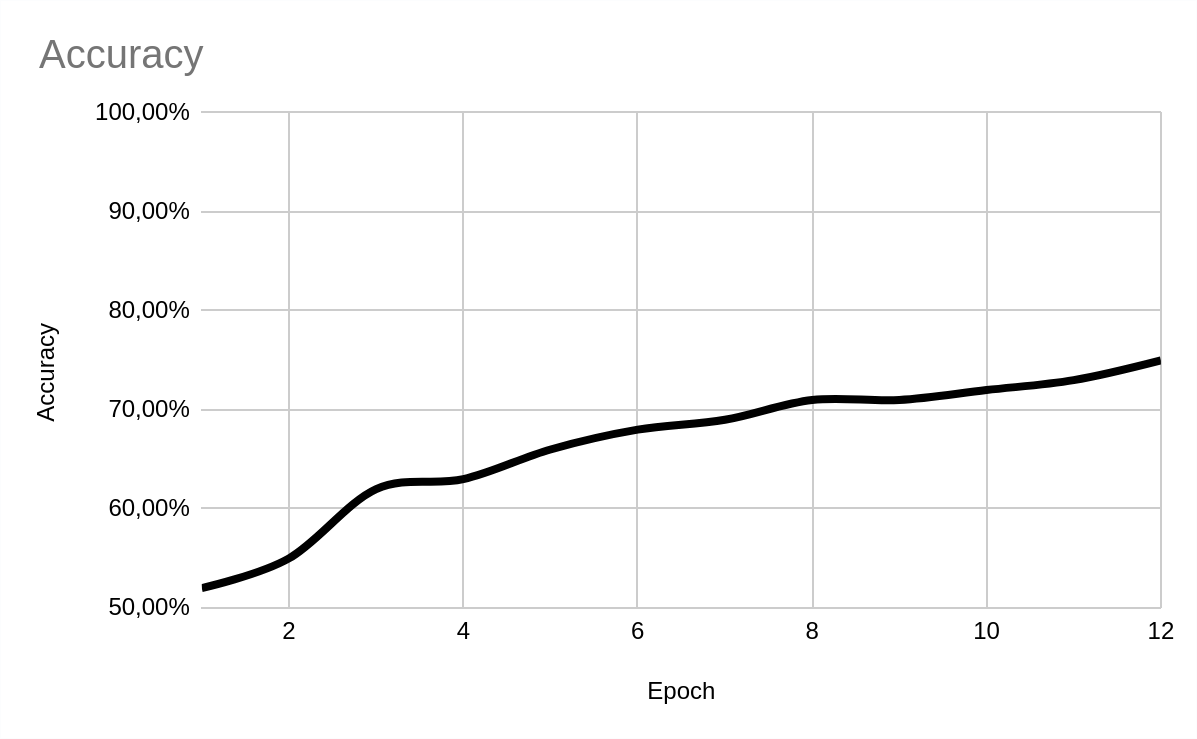
\includegraphics[scale=0.25]{accuracy1.png}
	\\\small Dokładność w kolejnych epokach uczenia
\end{center}

\hspace{1cm}Problem musi więc tkwić we wstępnym przetwarzaniu danych. Pojawił się błąd w interpretacji klas w danych źródłowych. Dostarczony opis problemu wskazywał na 18 klas decyzyjnych. Było to spowodowane faktem, że w danych rozróżniono wyraźnie skany osoby 'a' i osoby 'b', nawet, jeżeli osoby te wykonywały ten sam gest. Oznaczało to, że aby osiągnąć docelową dokładność, klasyfikator oprócz rozpoznawania gestów musiałby rozpoznawać osobę. Ilość klas została zredukowana do właściwej ilości, co znacząco poprawiło wyniki uczenia. Dodatkowo udało się wyznaczyć lepsze parametry sieci - lepszy współczynnik uczenia i mniejsza liczba neuronów w warstwie ukrytej (150).

\begin{center}
	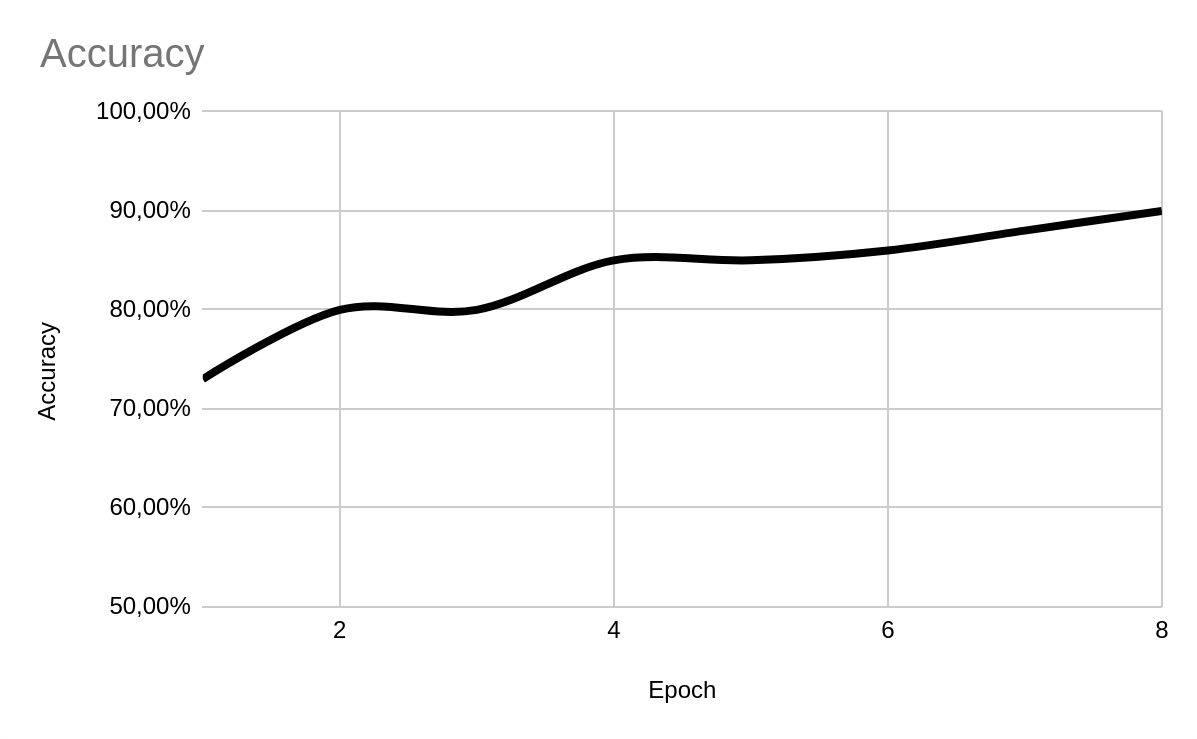
\includegraphics[scale=0.25]{accuracy2.png}
	\\\small Dokładność w kolejnych epokach uczenia
\end{center}

\hspace{1cm}Oprócz wzrostu dokładności, zmalała też ilość epok uczenia potrzebnych do jej osiągnięcia. Dokładność 90\% jest już zadowalającym wynikiem i jest osiągana średnio w ciągu 8 epok. Zaimplementowano już wersję klasyfikatora z dwiema warstwami ukrytymi, ale nie przeprowadzono jeszcze testów na tych danych. Spodziewamy się dodatkowego poprawienia wyników.

\section{Komentarze i wnioski}
\hspace{1cm}W pierwszej wersji udało się utworzyć klasyfikator zdolny do uczenia, niestety drobne niedociągnięcia i przeoczenia spowodowały brak wysokich wyników. Problem zidentyfikowano i rozwiązano, co pozwoliło osiągnąć klasyfikację o dokładności dochodzącej do 90\%.\\
\hspace{1cm}Największym problemem napotkanym podczas pierwszych etapów badań był jednak brak jednoznacznej interpretacji rekordów nie mających etykiet w plikach wejściowych. Ostatecznie zostały one pominięte w podstawowej klasyfikacji i trafiły na listę potencjalnych eksperymentów do wykonania po zrealizowaniu podstawy projektu. Płynie z tego wniosek, że podczas tworzenia zbiorów danych rozbitych na pojedyncze pliki należy pamiętać o właściwym oznaczaniu etykiet, aby nie doszło do niejednoznaczności.\\
\hspace{1cm}Obecne wyniki zostały osiągnięte bez finalnej wersji modelu klasyfikatora. Przy tak takiej ilości danych wejściowych sieci, dodatkowa warstwa ukryta może poprawić wyniki. W kolejnej wersji raportu spodziewamy się poprawionych wyników. Dodatkowo do zaimplementowania został mechanizm importu/eksportu wyuczonego modelu do/z pliku, ale przez fakt, że uczenie nie trwa długo, nie jest to zadanie o wysokim priorytecie.

\end{document}